\chapter{Astrolabium}

In dit hoofdstuk ga je aan de slag met het \textit{astrolabium}, een van de oudste navigatie-instrumenten. Je gebruikt het astrolabium zoals in figuur \ref{astrolabe-face}\textcolor{red}{ref?}. Er bestaan twee varianten van het astrolabium, het sterrenkundig astrolabium en het zeemansastrolabium, dat versimpeld was en makkelijker te gebruiken op het dek van een schip. Het astrolabium dat wij gebruiken is een sterrenkundig astrolabium.

Je bouwt eerst je eigen astrolabium, daarvoor krijg je een werkblad met de onderdelen van het astrolabium uitgedeeld. Allereerst kijken we naar de achterkant van het astrolabium (figuur \ref{astrolabe-back}).

De ringen, van buiten naar binnen, geven het volgende weer:
\begin{itemize}
 \item Schaal om de hoogte van een ster te bepalen.
 \item Dagen van de sterrenbeelden.
 \item Namen van de sterrenbeelden (de tekens van de dierenriem).
 \item Kalender passend bij het jaar 1394 (deze loopt negen dagen voor op de kalender voor onze tijd).
 \item Kalender passend bij onze eigen tijd. Deze kun je inkleuren met kleurpotlood of highlighter om aan te geven dat dit de kalender is die je moet gebruiken.
 \item In de volgende twee ringen worden traditioneel de naamdagen van katholieke of anglicaanse heiligen weergegeven. Deze zijn weggelaten in ons astrolabium.
 \item De binnenste ring (schaduwschaal) zullen we niet gebruiken.
\end{itemize}

\begin{figure}[!b]
\centering
 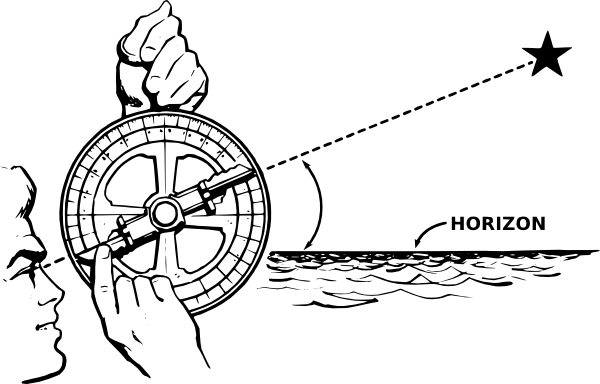
\includegraphics[width=0.7\textwidth]{astrolabe-hi.png}
 \label{astrolabe-face}
 \caption{Zo houdt je het astrolabium vast.}
\end{figure}

\begin{figure}
\centering
 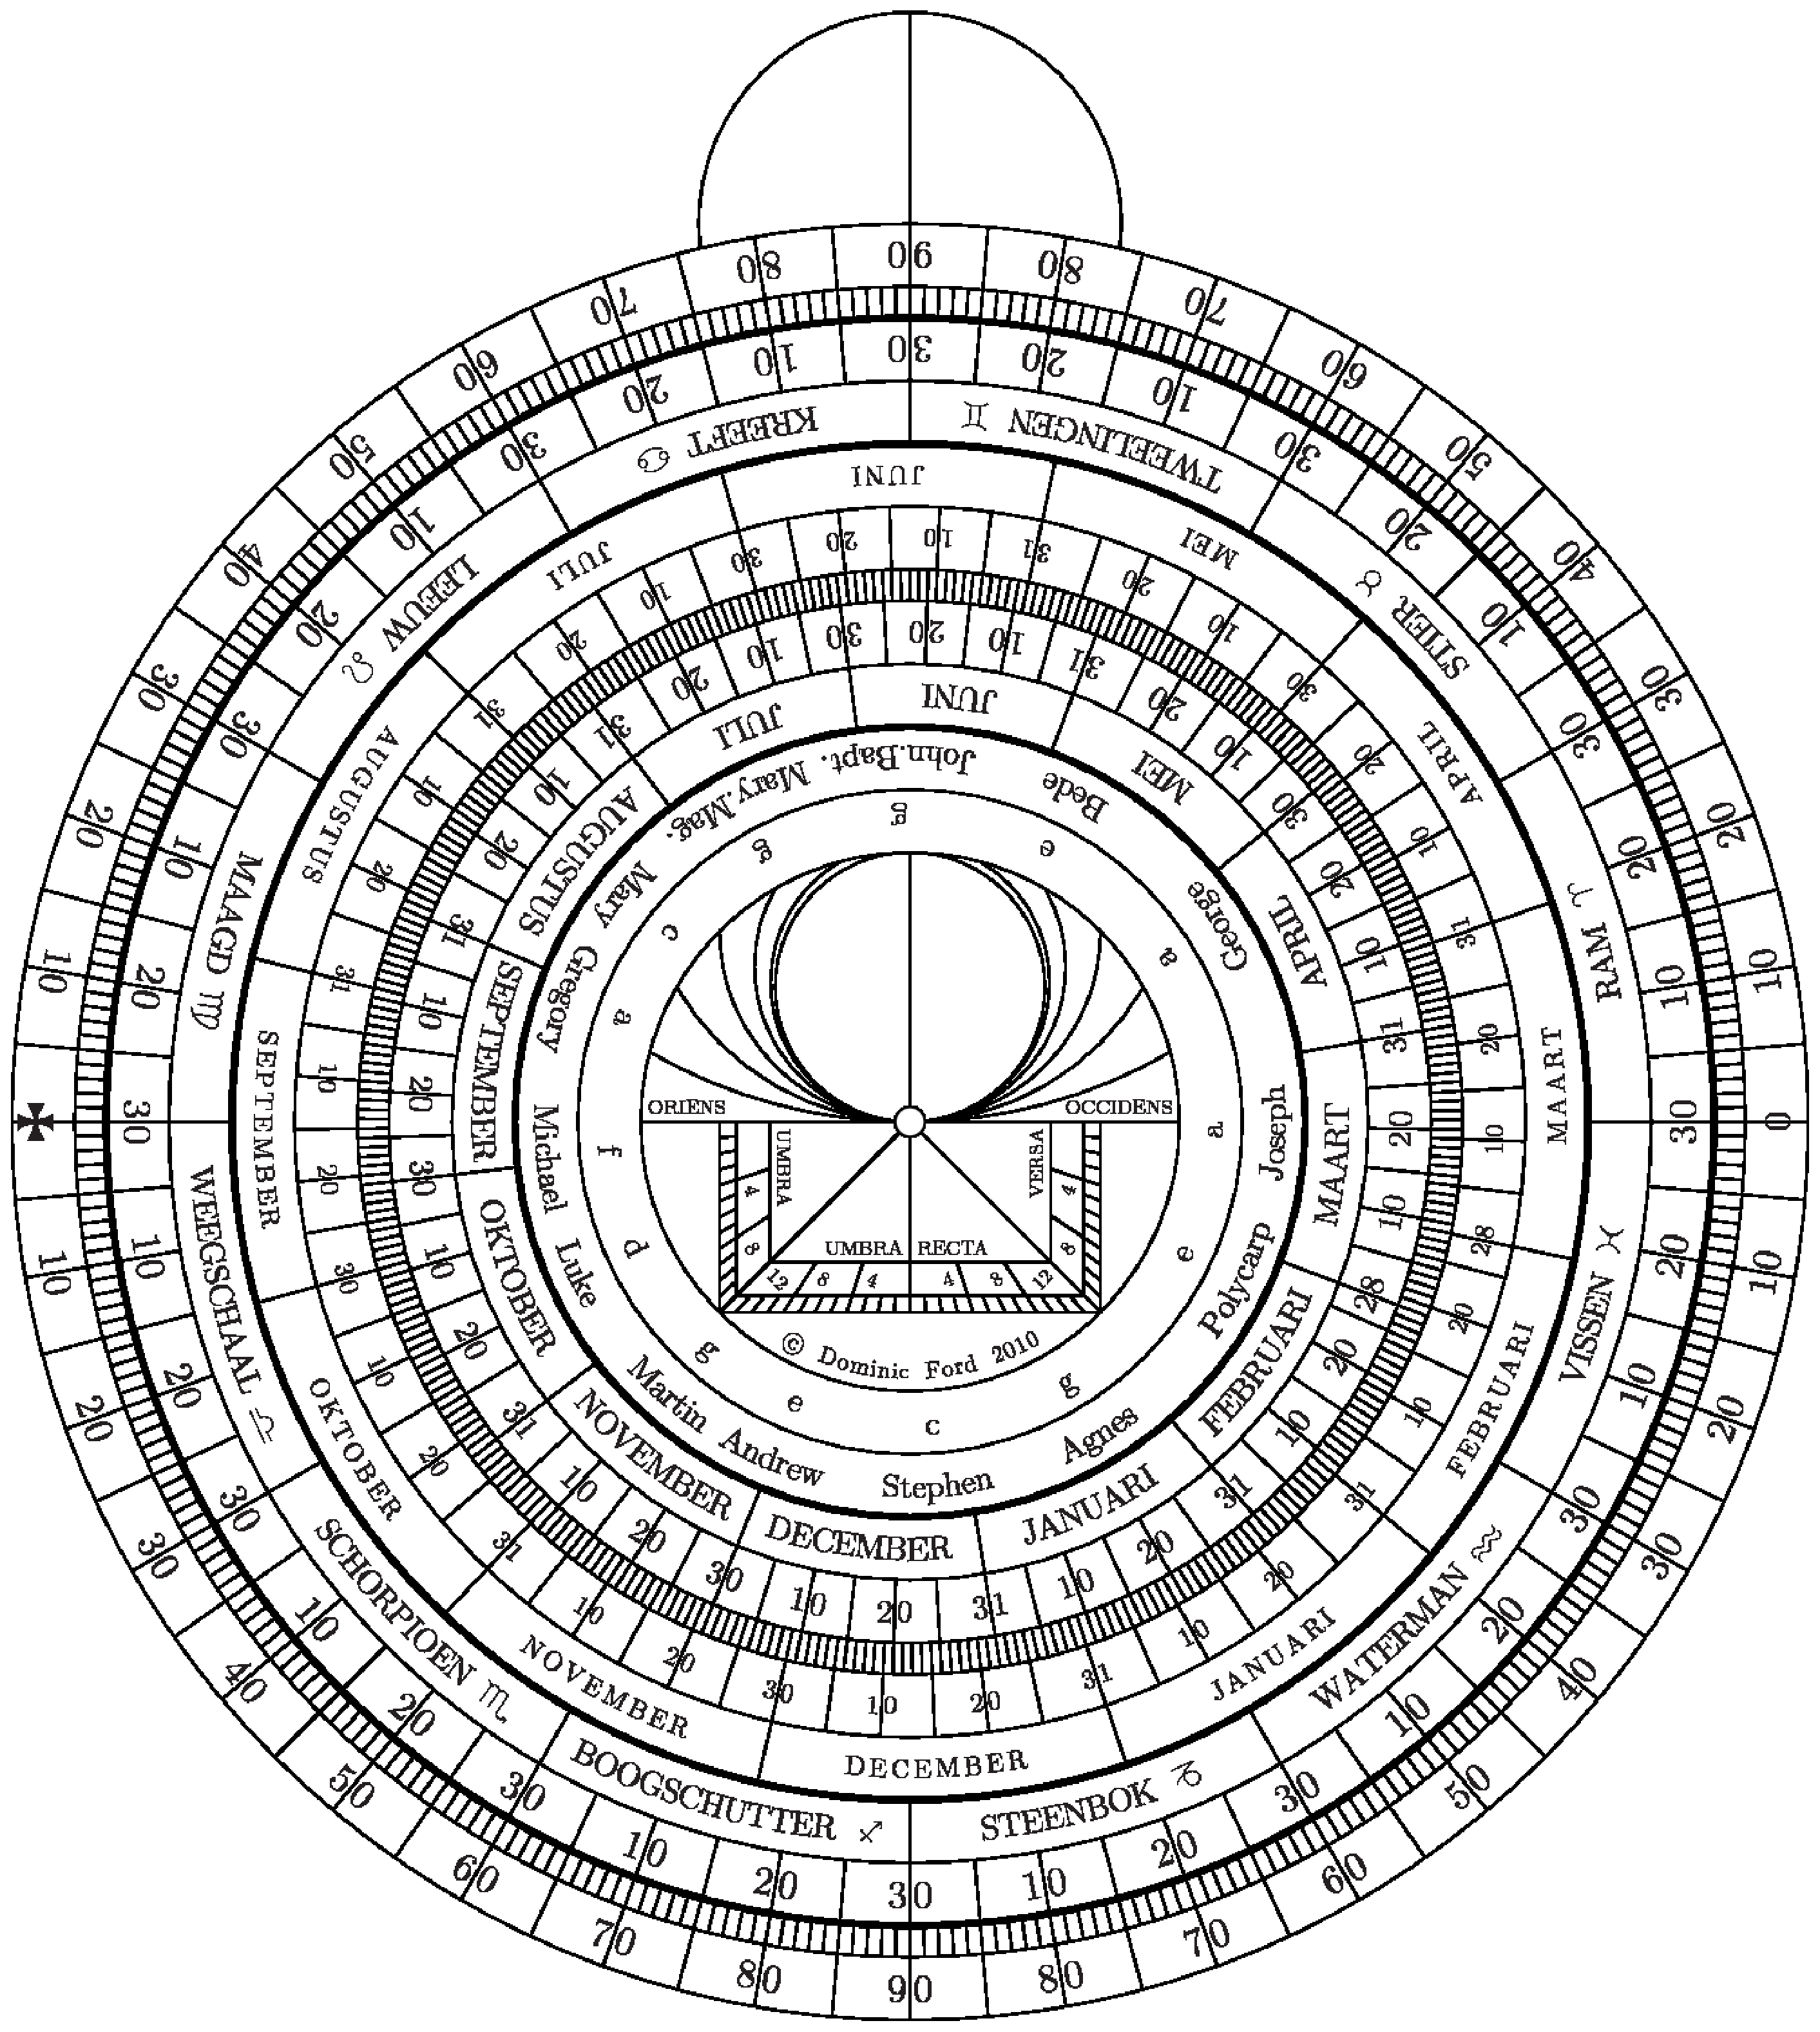
\includegraphics[width=0.7\textwidth]{astrolabiumNL/mother_back.eps}
 \label{astrolabe-back}
 \caption{De achterkant van het astrolabium}
\end{figure}

De wijzer (alidade) (figuur \ref{alidade} \textcolor{red}{ref?}) draait over de achterkant van het astrolabium. \textcolor{red}{Naast de alidade op je werkblad wordt ook de \textit{rule} afgebeeld. Deze zullen we niet gebruiken.}

\begin{figure}
\centering
 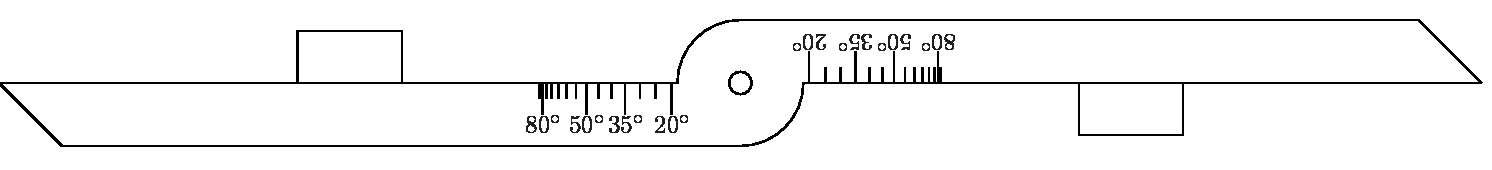
\includegraphics[width=0.7\textwidth]{astrolabiumNL/alidade}
 \label{alidade}
 \caption{De alidade}
\end{figure}

De voorkant van het astrolabium heeft het alfabet (de letters J, V en W ontbreken) en een gradenboog rondom de \textit{plaat}. De plaat is gemaakt voor 52$^\circ$ Noorderbreedte, de breedtegraad van Nederland. Voor een andere breedtegraad heb je een andere plaat nodig. Het alfabet geeft de tijd aan, het kruis \kreuz\ is middernacht, de \textbf{A} is \'e\'en uur, de \textbf{M} is 12 uur 's middags, enzovoort.

Op de plaat zie je cirkels rondom een punt dat niet het middelpunt van het astrolabium is. Dit punt heet het \textit{zenit}, en het geeft het punt recht boven je hoofd (als je rechtop staat) weer. Eromheen zijn de cirkels genaamd \textit{almucantaren}. De almucantaar die gemarkeerd is met $0^\circ$ is de \textit{horizon}. De verticale lijn tussen de \textbf{M} en \kreuz\ is de noord-zuid meridiaan (het zuiden ligt bij \textbf{M}), en de lijn tussen \textbf{S} en \textbf{F} is de oost-west lijn. \textcolor{red}{Te veel tekst, onderbreek met een knipvraag}

Het laatste onderdeel, gemaakt van doorzichtig plastic, maar in vroeger tijden vaak een gouden of koperen plaat met veel uitsparingen, is de \textit{spin} (op het werkblad heet dit de \textit{r\`ete}, maar in het Nederlands is het de spin). Op de spin staan een sterrenkaart en uren afgebeeld. De cirkel met daarin de namen van de sterrenbeelden is het \textit{zonnepad}. Ook staan er drie cirkels op afgebeeld. De buitenste (aan de rand van de spin) geeft de Steenbokskeerkring aan (dit is een parallel op $23,5^{\circ}$ zuiderbreedte).  De kleinere cirkel is de evenaar, en de kleinste cirkel (gedeeltelijk bedekt door het zonnepad) is de Kreeftskeerkring (de parallel op $23,5^{\circ}$ noorderbreedte). Als je de spin met de klok mee draait, zie je de sterren opkomen in het oosten en ondergaan in het westen.

De voorkant en de achterkant zijn niet helemaal cirkelvormig: aan de bovenkant zit nog een ring waaraan je het astrolabium kan vasthouden.

\begin{opgave}[\schaar]
 Knip nu alle onderdelen van het astrolabium uit. Lijm de voorkant en de achterkant op elkaar zodat de ring van beide onderdelen op elkaar zit, en je alle tekst kan lezen. Met een splitpen bevestig je de alidade op de achterkant en de spin op de voorkant van het astrolabium.
\end{opgave}

\section{Bepaal de breedtegraad met het astrolabium}
Het bepalen van de breedtegraad met het astrolabium is niet moeilijk, je gebruikt slechts een klein deel van de mogelijke metingen die je met het astrolabium kan doen. Je kan dit ook doen met simpeler instrumenten zoals de sextant, de octant of de Jakobsstaf, het principe is hetzelfde. Je kan zo'n instrument zelf knutselen met een geodriehoek of gradenboog en een rietje om doorheen te kijken.

Als je 's nachts de breedtegraad wil bepalen, gebruik je de Poolster. Deze kun je vinden door eerst het sterrenbeeld Grote Beer (Ursa Major) te vinden. In Nederland wordt deze ook wel het Steelpannetje genoemd. Bekijk ook de figuur \ref{poolster} hieronder om de Poolster te vinden:
\begin{figure}[h]
\centering
 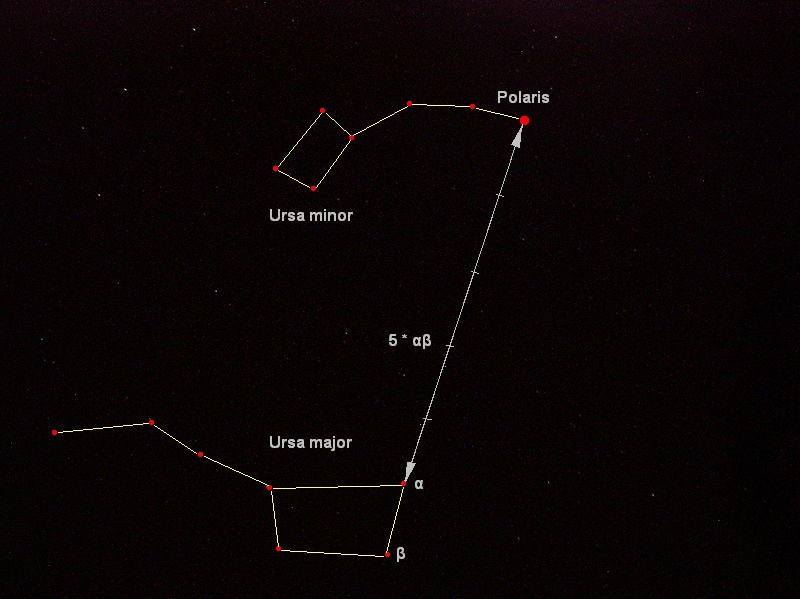
\includegraphics[width=0.6\textwidth]{Polaris.jpg}
 \label{poolster}
 \caption{Vind de Poolster met behulp van de Grote Beer.}
\end{figure}

Als je de Poolster hebt gevonden, kun je als volgt de hoogte bepalen: houd het astrolabium aan de ring vast, zodat het vrij hangt voor je. Draai de wijzer zodat je precies langs de wijzer naar de Poolster kijkt (de ster moet precies tussen de flapjes van de wijzer zichtbaar zijn). Op de buitenste schaalverdeling aan de achterkant van het astrolabium kun je nu zien hoe hoog de Poolster staat. Dit is de breedtegraad.

\begin{opgave}
Maak een tekening van deze situatie: laat zien hoe de aarde, de waarnemer, het astrolabium en de ster zich bevinden ten opzichte van elkaar. Leg nu uit waarom de breedtegraad en de hoogte van de Poolster hetzelfde zijn.
\begin{hint}
 Bedenk dat, op de Noordpool, de Poolster recht boven je staat en op de evenaar de Poolster precies op de horizon staat.
\end{hint}
\end{opgave}

\textbf{Herinnering: } kijk nooit recht in de zon!
\begin{opgave}[\schaar]
 \label{astrolabium:breedtegraad}
 Sta met je rug naar de zon toe. Houd het astrolabium aan de ring vast, voor je, zodat het vrij hangt. Draai de wijzer zodat het evenwijdig is met de zonnestralen - de flapjes mogen geen schaduw geven. Nu kun je op de buitenste schaalverdeling aan de achterkant de hoogte van de zon aflezen. 
 \begin{subopgave}
  Wat is de hoogte van de zon?
 \end{subopgave}
\end{opgave}

\begin{opgave}
 Waarom is het belangrijk dat je de maximale hoogte van de zon bepaalt?
\end{opgave}

\begin{opgave}
 Op het midden van de dag staat de zon op het hoogste punt - en precies in het Zuiden. Als je de maximale hoogte van de zon bepaald hebt, is dat echter niet hetzelfde als de breedtegraad. Waarom niet?
 \begin{hint}
  Vergelijk de positie van de zon met de positie van de Poolster.
 \end{hint}
\end{opgave}

\begin{opgave}
 Hoe vind je dan wel de breedtegraad, als je de maximale hoogte van de zon weet?
 \begin{antwoord}
  Breedtegraad $= 90^{\circ} -$ hoogte(zon)
 \end{antwoord}
\end{opgave}

\begin{opgave}
 Meet de breedtegraad met je astrolabium.
 \begin{subopgave}
  Wat is de uitkomst van je meting?
 \end{subopgave}
 \begin{subopgave}
  Heino ligt op $52,4$ graden Noorderbreedte. Wat is het verschil met jouw meting? Hoe denk je dat dit verschil veroorzaakt wordt?
 \end{subopgave}
\end{opgave}


\section{Tijdsbepaling met het astrolabium}

Op de spin zie je een ring met de namen van de twaalf sterrenbeelden van de dierenriem. Ieder sterrenbeeld hoort bij bepaalde data in het jaar:

\begin{center}
\begin{tabular}{|l|l|}
 \hline
 Sterrenbeeld & Data \\
 \hline
 Ram & 21 maart -- 21 april \\
 Stier & 21 april -- 21 mei \\
 Tweelingen & 21 mei -- 21 juni \\
 Kreeft & 21 juni -- 21 juli \\
 Leeuw & 21 juli -- 21 augustus \\
 Maagd & 21 augustus -- 21 september \\
 Weegschaal & 21 september -- 21 oktober \\
 Schorpioen & 21 oktober -- 21 november \\
 Boogschutter & 21 november -- 21 december \\
 Steenbok & 21 december -- 21 januari \\
 Waterman & 21 januari -- 21 februari \\
 Vissen & 21 februari -- 21 maart \\
 \hline
\end{tabular}
\end{center}

Je hoeft deze tabel niet uit je hoofd te leren, je kan namelijk op de achterkant van het astrolabium zien welk sterrenbeeld bij welke datum hoort. Let op dat je de binnenste kalender gebruikt! We gaan nu eerst het tijdstip van zonsopgang en zonsondergang van vandaag bepalen. 
\begin{opgave}
 Gebruik een stift of highlighter om, op het zonnepad (op de spin) een stip te zetten bij de datum van vandaag. Dit stipje is de zon. Nu draai je de spin zodat de zon op de oostelijke horizon ligt (dus op de linkerhelft van de plaat). De lijn die door het midden van de plaat en de zon gaat wijst nu een letter op de buitenrand van de plaat aan. Deze letter geeft het uur van zonsopgang aan. Hoe laat is dit?
 \begin{hint}
  Kamp is 13 tot 17 augustus 2018, je zet dus een stipje tussen het midden en het einde van de Leeuw op het zonnepad. Vergeet niet om te rekenen naar zomertijd.
 \end{hint}
 \begin{antwoord}
  $6:24$.
 \end{antwoord}
\end{opgave}

\begin{opgave}
 Bereken nu op dezelfde manier het tijdstip van zonsondergang vandaag. Gebruik hiervoor de westelijke horizon (de rechterkant van het astrolabium). 
 \begin{antwoord}
  $21:05$.
 \end{antwoord}
\end{opgave}

We gaan nu het tijdstip bepalen. Hiervoor is het belangrijk dat je niet recht in de zon kijkt!
\begin{opgave}
 Bepaal de hoogte van de zon, op dezelfde manier als je deed bij het bepalen van de breedtegraad (opgave \ref{astrolabium:breedtegraad})
 \begin{subopgave}
 Wat is de hoogte van de zon?
 \end{subopgave}
 Draai nu de spin zo dat het stipje op de almucantaar (de gebogen lijnen op de plaat, zie ook de uitleg in het begin van dit hoofdstuk) met dezelfde hoogte staat. Bepaal nu de hoek tussen de zon en de noord-zuid meridiaan. Het tijdstip wordt nu gegeven door de volgende formule:
 \[ \textrm{Tijdstip} = 12 \pm \frac{24\times\textrm{hoek}}{360} \]
 waarbij de $\pm$ betekent dat je moet optellen als het middag is, maar aftrekken als het ochtend is.
 \begin{subopgave}
  Hoe laat is het volgens deze formule?
 \end{subopgave}
 \begin{subopgave}
  Reken dit om naar zomertijd. Klopt het met de tijd op de klok?
 \end{subopgave}
\end{opgave}

\begin{opgave}[\discussie]
 Je hebt in de vorige opgave de hoek tussen de zon en het zuiden bepaald. Wijs nu de richting van het zuiden aan. Ben je het eens met je groepje? Verschillen jullie antwoorden meer of minder dan in het horlogepracticum?
\end{opgave}

\begin{opgave}
 In de bovenstaande opgaven zijn we uitgegaan van het noordelijk halfrond. Wat moet je aanpassen voor het zuidelijk halfrond?
 \begin{antwoord}
  Je hebt een spin nodig met de sterrenkaart van het zuidelijk halfrond, dus met Sigma Octantis in plaats van de Poolster. Ook heb je voor iedere breedtegraad een andere plaat nodig.
 \end{antwoord}

\end{opgave}

\section{Bepaal de lengtegraad met het astrolabium}
Stel je nu voor dat je de navigator op een $17^e$-eeuws schip bent. 
\begin{opgave}
 Wat kan er mis gaan op een schip als de navigator niet de precieze lengtegraad weet?
 \begin{antwoord}
  Veel mogelijkheden, maar de belangrijkste is dat de navigator kan denken dat het schip in open water vaart, terwijl het in werkelijkheid in ondiep water vaart en op een rif kan lopen.
 \end{antwoord}
\end{opgave}

\begin{opgave}
 Een primitieve techniek om de lengtegraad te bepalen ging uit van de snelheid van het schip. Zeelieden gebruikten een touw met knopen erin, die ze vanaf de achterkant van het schip naar beneden lieten, en dan met een zandloper maten ze de hoeveelheid knopen die in een bepaalde tijd in het water verdween.
 \begin{subopgave}
  Wat is het probleem met deze techniek?
  \begin{antwoord}
   Als je tegen de stroming invaart, meet je een hogere snelheid dan het schip daadwerkelijk vaart. Als je met de stroming meevaart, meet je een lagere snelheid. In een storm is de techniek compleet onbruikbaar.
  \end{antwoord}
 \end{subopgave}
 \begin{subopgave}
 Kun je een betrouwbare manier bedenken om de snelheid te bepalen, met technieken die in de $17^e$ eeuw of eerder beschikbaar waren?
 \begin{antwoord}
  Nee.
 \end{antwoord}
 \end{subopgave}
\end{opgave}

\begin{opgave}
Omdat de aarde iedere dag volledig om zijn as draait, ziet een waarnemer op lengtegraad A gedurende een dag dezelfde sterren als een waarnemer op lengtegraad B (zolang de lucht niet bewolkt is en de breedtegraden gelijk zijn). Ziet waarnemer A om middernacht, lokale tijd, dezelfde sterren op hetzelfde tijdstip als waarnemer B om middernacht, lokale tijd?
\begin{antwoord}
 Ja
\end{antwoord}
\end{opgave}

\begin{opgave}
Hoeveel graden draait de aarde in \'e\'en uur?
\begin{antwoord}
 $\frac{360^{\circ}}{24 \textrm{ uur}} = 15^{\circ}$.
\end{antwoord}
\end{opgave}

\begin{opgave}
 Als je nu op een schip bent, je weet niet waar, en je weet de precieze tijd op de nulmeridiaan (de meridiaan die door Greenwich/Londen loopt), kun je dan de lengtegraad van je eigen locatie bepalen met het astrolabium? Hoe?
 \begin{antwoord}
  Met het astrolabium bepaal je de lokale tijd. De tijd op de nulmeridiaan is gegeven, dus je kan het tijdsverschil berekenen. Het tijdsverschil in uren kun je dan vermenigvuldigen met 15 om het verschil in lengtegraden te bepalen.
 \end{antwoord}
\end{opgave}

\begin{opgave}
 Vraag je begeleider om de precieze tijd in Greenwich op te zoeken. Bepaal nu de tijd en lengtegraad in Heino met je astrolabium.
 \begin{hint}
  GMT kun je vinden op deze website: \texttt{https://time.is/GMT}.
 \end{hint}
\begin{antwoord}
 de lengtegraad van Heino is 6.2 graden oosterlengte
\end{antwoord}
\end{opgave}

In 1735 vond John Harrison een betrouwbare scheepsklok uit, maar pas in 1800 hadden de meeste schepen een goede klok aan boord.
\begin{opgave}
 Leg in je eigen woorden uit waarom het belangrijk is een betrouwbare klok aan boord van een schip te hebben.
\end{opgave}


\newpage